\documentclass[a4paper]{article}

\usepackage[czech]{babel} %https://github.com/michal-h21/biblatex-iso690
\usepackage[
   backend=biber      % if we want unicode 
  ,style=iso-numeric % or iso-numeric for numeric citation method          
  ,babel=other        % to support multiple languages in bibliography
  ,sortlocale=cs_CZ   % locale of main language, it is for sorting
  ,bibencoding=UTF8   % this is necessary only if bibliography file is in different encoding than main document
]{biblatex}

\usepackage[utf8]{inputenc}
\usepackage{fancyhdr}
\usepackage{amsmath}
\usepackage{amssymb}
\usepackage[left=2cm,right=2cm,top=2.5cm,bottom=2.5cm]{geometry}
\usepackage{graphicx}
\usepackage{pdfpages}
\usepackage{url}

\usepackage{siunitx}
\sisetup{locale = DE}  %, separate-uncertainty = true    kdybych chtel +/-

\usepackage{float}
\newfloat{graph}{htbp}{grp}
\floatname{graph}{Graf}
\newfloat{tabulka}{htbp}{tbl}
\floatname{tabulka}{Tabulka}

\renewcommand{\thefootnote}{\roman{footnote}}

\pagestyle{fancy}
\lhead{Praktikum III - (13) Vlastnosti rentgenového záření}
\rhead{Vladislav Wohlrath}
\author{Vladislav Wohlrath}

\bibliography{source}

\begin{document}

\begin{titlepage}
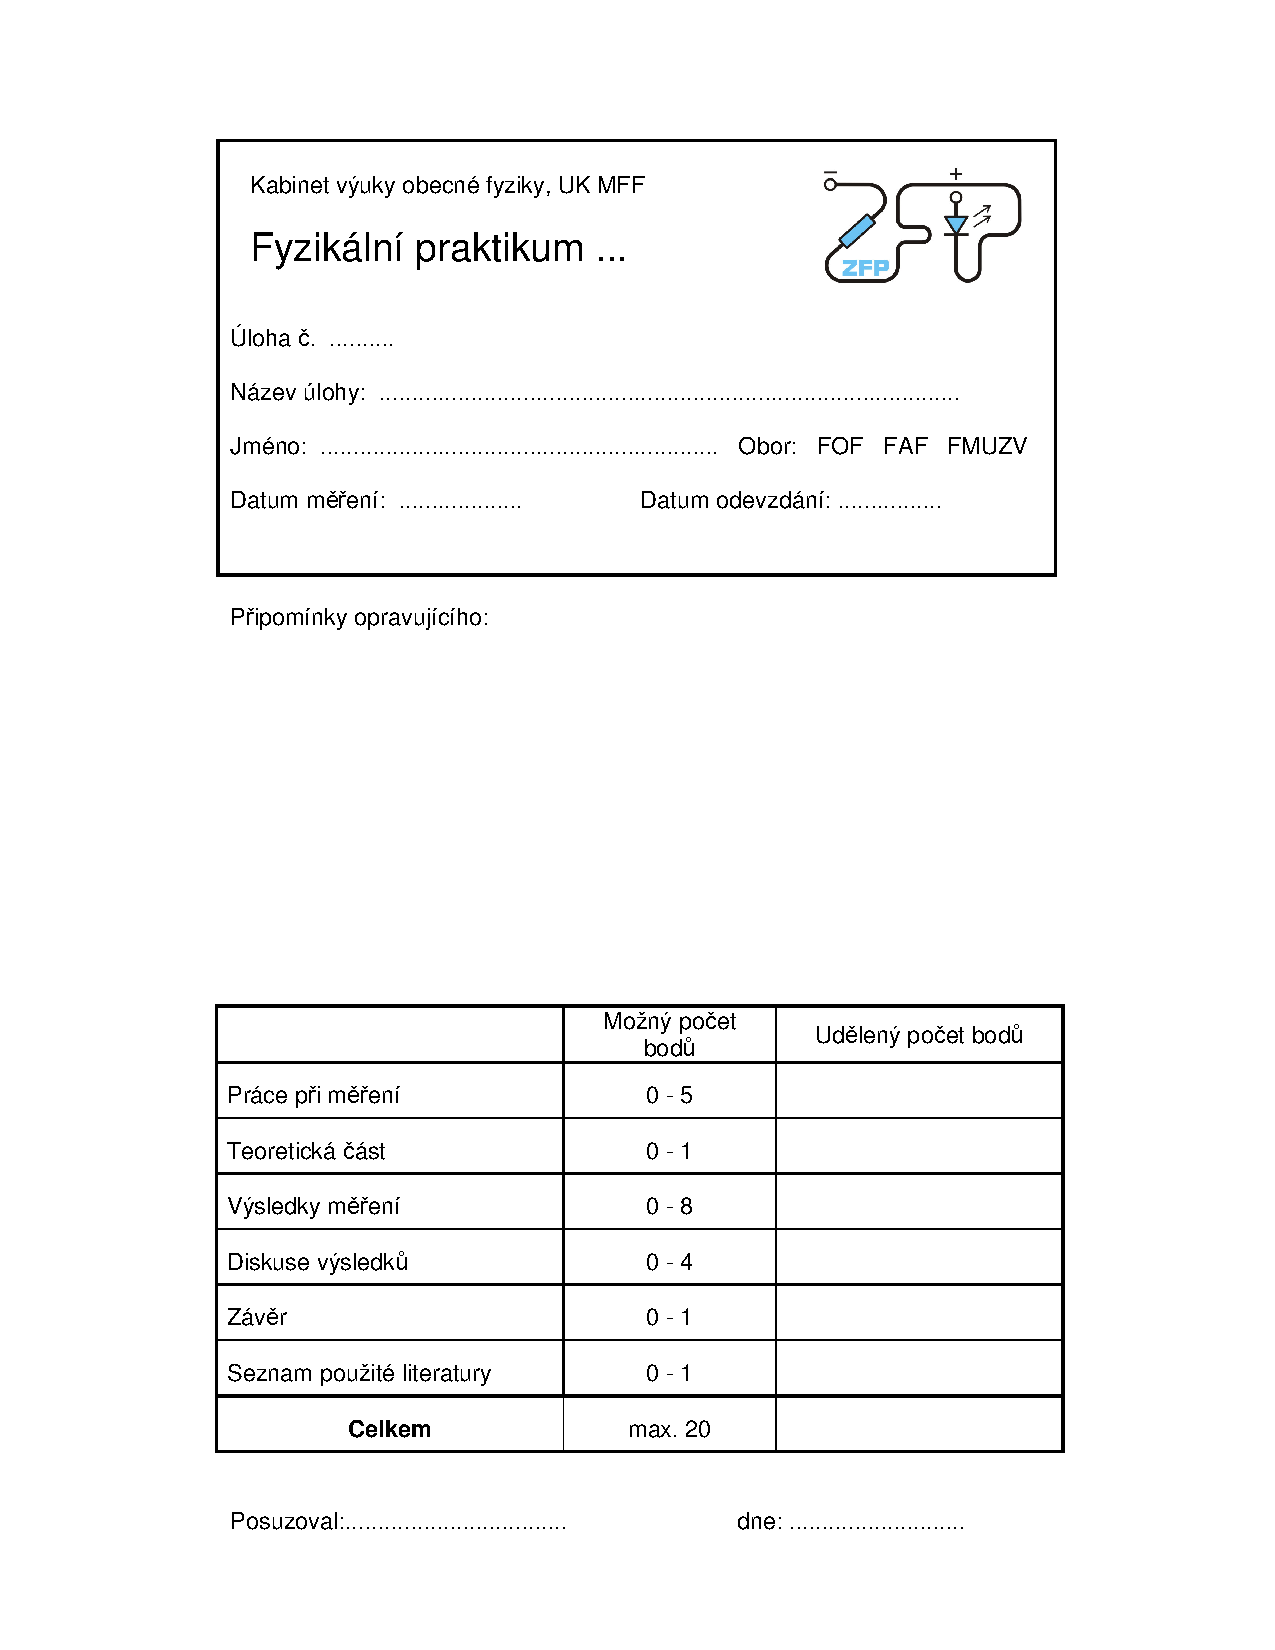
\includepdf[pages={1}]{./graficos/tit.pdf}
\end{titlepage}

\section*{Pracovní úkoly}
\begin{enumerate}
\item Ze zadané hustoty krystalu fluoridu lithného určete vzdálenost $d$ hlavních atomových rovin.
\item Proměřte úhlovou závislost intenzity difraktovaného rentgenového záření při pevné orientaci krystalu.
\item Proměřte spektrum rentgenového záření při konstantním anodovém napětí rentgenky $U_a = \SI{20}{\kilo\volt}$.
\item Z mezní hodnoty energie spojitého spektra určete Planckovu konstantu, porovnejte s tabelovanou hodnotou. Určete vlnové délky čar $K_\alpha$, $K_\beta$ (porovnejte s tabelovanými hodnotami), spočtěte jejich vlnočty a odpovídající energetické rozdíly vyjádřete v \si{\keV}. Určete konstanty stínění.

\end{enumerate}

%Teoretická část
\section*{Teoretická část}

%Výsledky měření
\section*{Výsledky měření}

%Diskuze výsledků
\section*{Diskuze}
Úhlová závislost intenzity při pevné orientaci krystalu dopadla podle očekávání. Většina záření se difraktuje pod úhlem rovným úhlu dopadu.


Vlnové délky pozorovaných spektrálních čar se v rámci standardní odchylky neshodují s tabelovanými hodnotami $\lambda_{\alpha t} = \SI{154}{\pico\metre}$, $\lambda_{\beta t} = \SI{139}{\pico\metre}$, avšak v rámci $3\sigma$ už ano.

Námi změřená Planckova konstanta se shoduje s tabelovanou hodnotou \SI{6.626e-34}{\joule\s}.

Při určování mezních vlnových délek by bylo možné postupovat přesněji, kdybychom krátkovlnnou stranu spektra nafitovali přímkou a určili průsečík s nulou, místo toho abychom vzali nejkratší vlnovou délku, při které intenzita klesne pod určitou prahovou hodnotu. Stejně tak peaky od spektrálních čar by bylo možné nafitovat Gaussovou funkcí a jejich střed určit přesněji. Ještě větší přesnosti by se dalo dosáhnout přesnějším měřením úhlů a kratšími kroky v okolí těchto význačných vlnových délek. Proto jsme tento postup nepoužili.

%Závěr
\section*{Závěr}


\printbibliography[title={Seznam použité literatury}]

\end{document}